\begin{figure}[H]
\centering
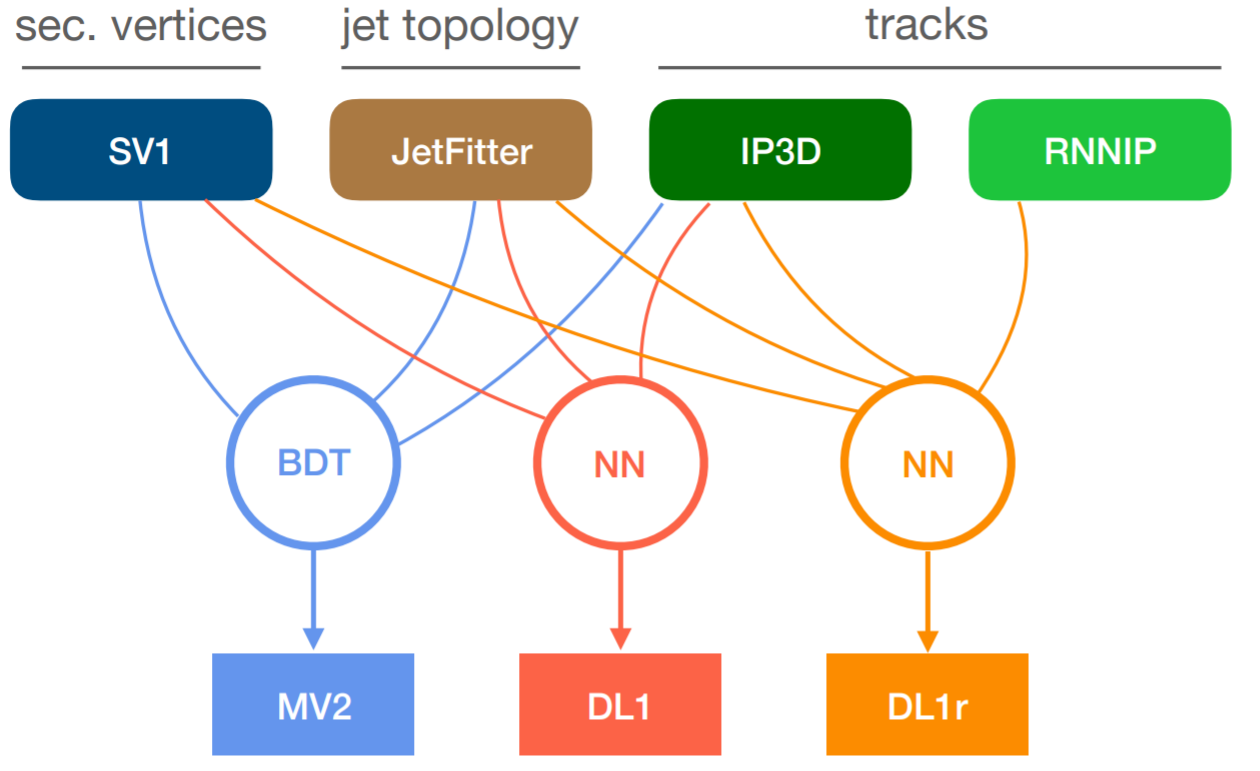
\includegraphics[width=\textwidth]{\FCNCFigures/screenshot/btaggers.png}
\caption{常用的b-tagger以及它们之间的关系。}
\label{fig:btaggers}
\end{figure}

\begin{figure}[H]
\centering
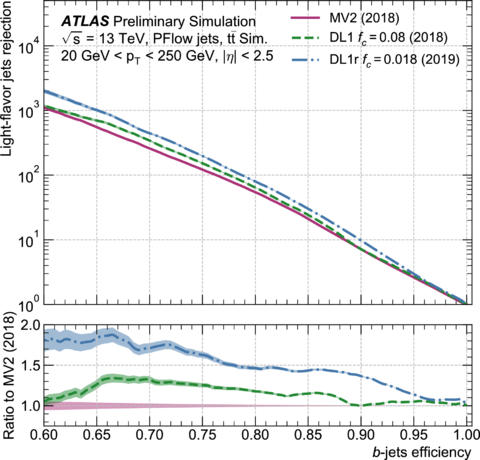
\includegraphics[width=0.49\textwidth]{\FCNCFigures/screenshot/btageff.png}
\caption{三种b-tag算法的ROC比较,最新的DL1r算法优于其他算法。}
\label{fig:btageff}
\end{figure}

\begin{figure}[H]
\centering
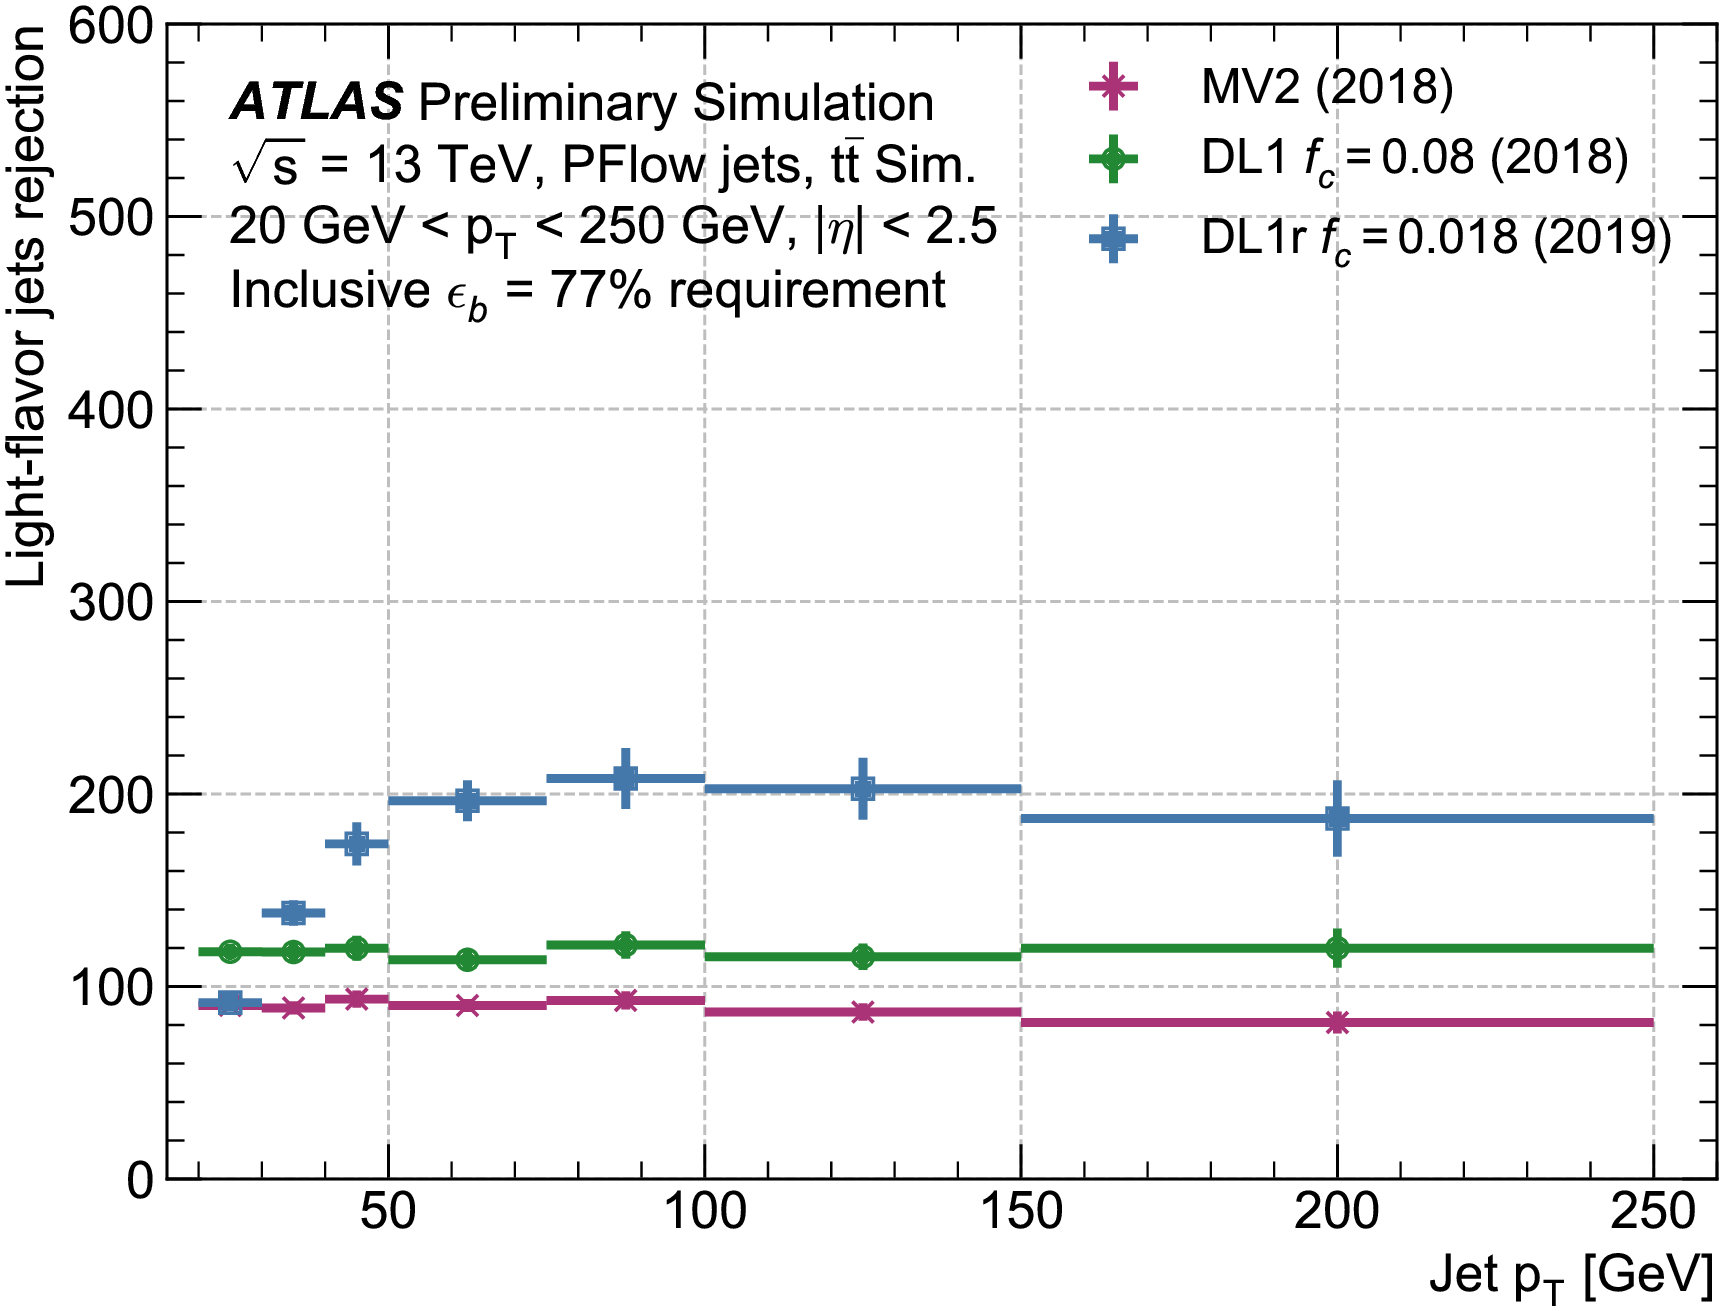
\includegraphics[width=0.49\textwidth]{\FCNCFigures/screenshot/btaglrej.png}
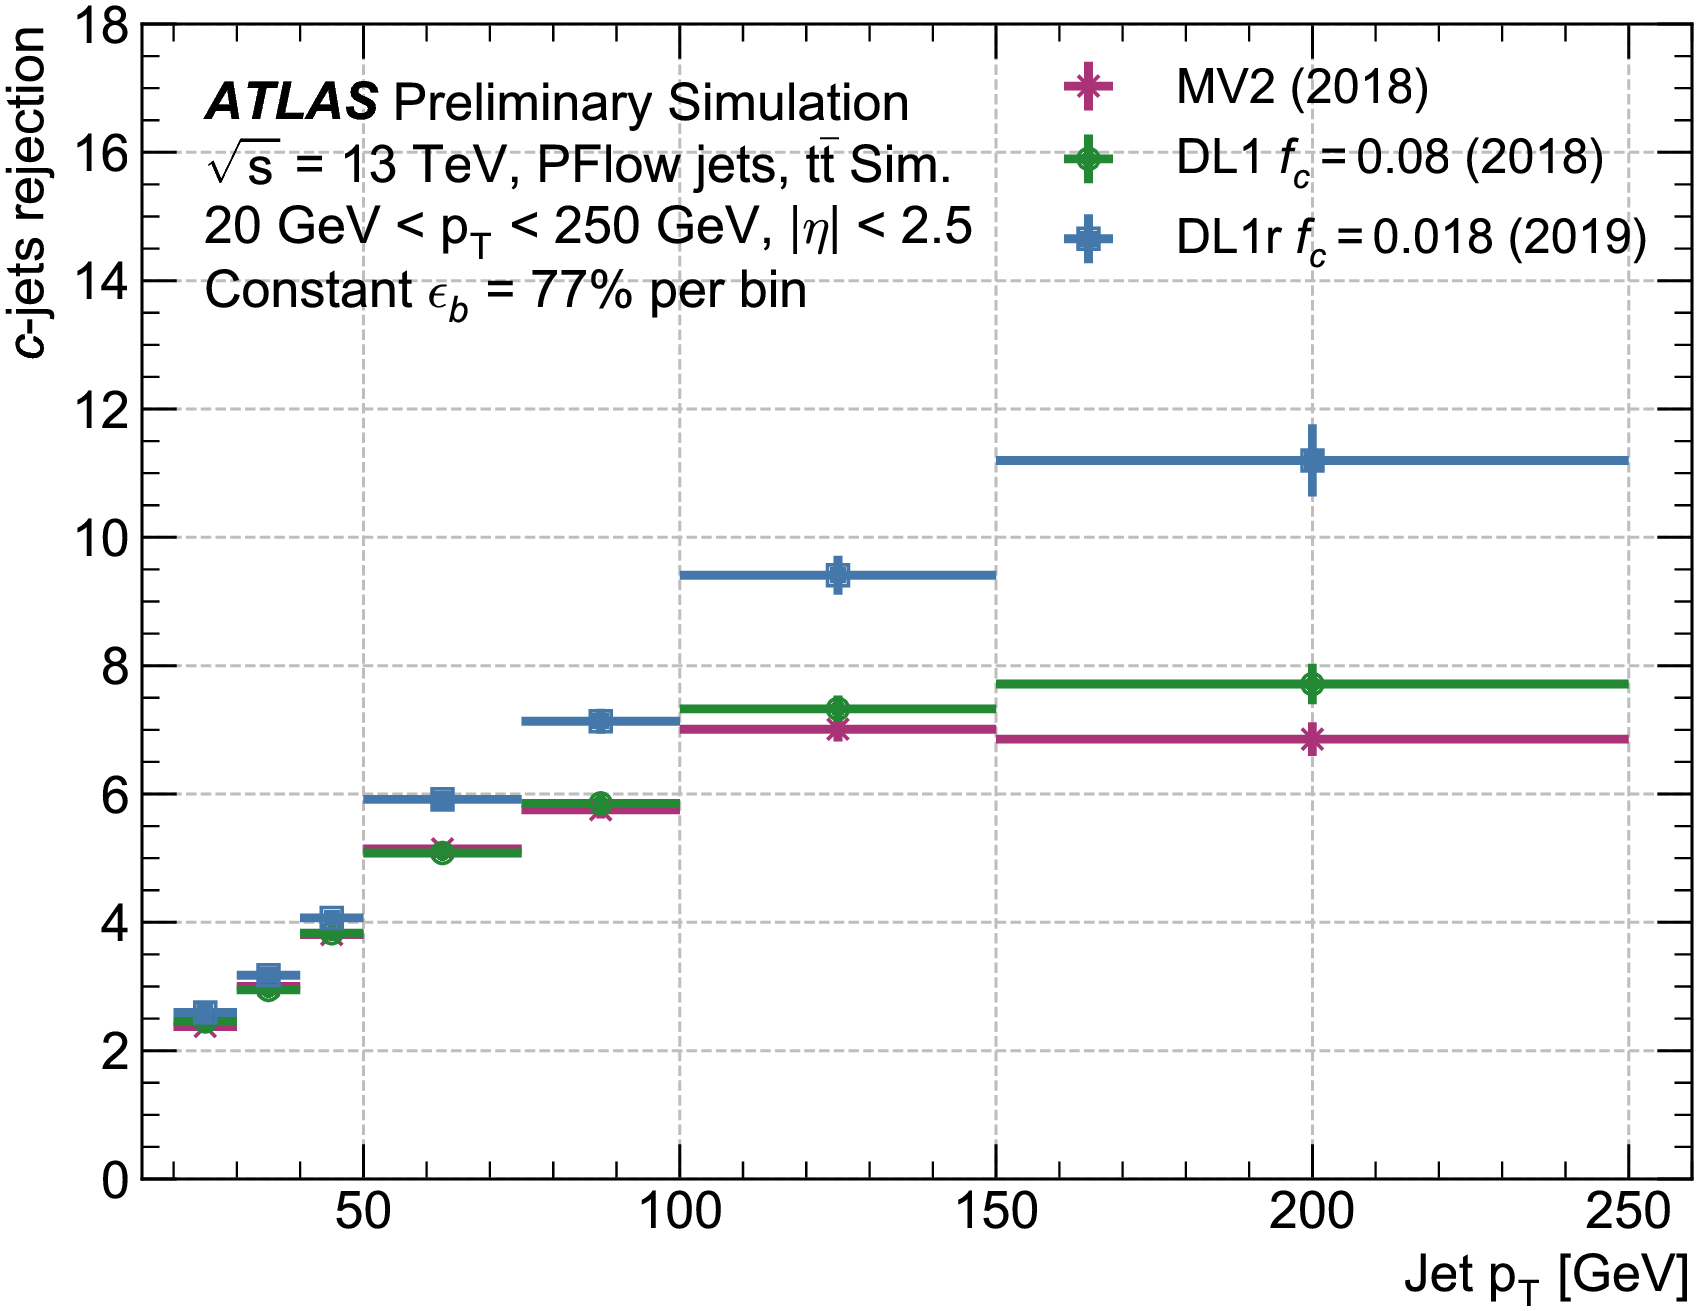
\includegraphics[width=0.49\textwidth]{\FCNCFigures/screenshot/btagcrej.png}
\caption{b-tag对轻味jet和带c的jet的拒绝率,可以看出对带c的jet的拒绝率远远低于轻味jet的拒绝率。}
\label{fig:btagrej}
\end{figure}